\documentclass{article}
\usepackage{tkz-graph}
\usepackage{paralist}
\pagestyle{empty}
\usetikzlibrary{patterns}

\begin{document}

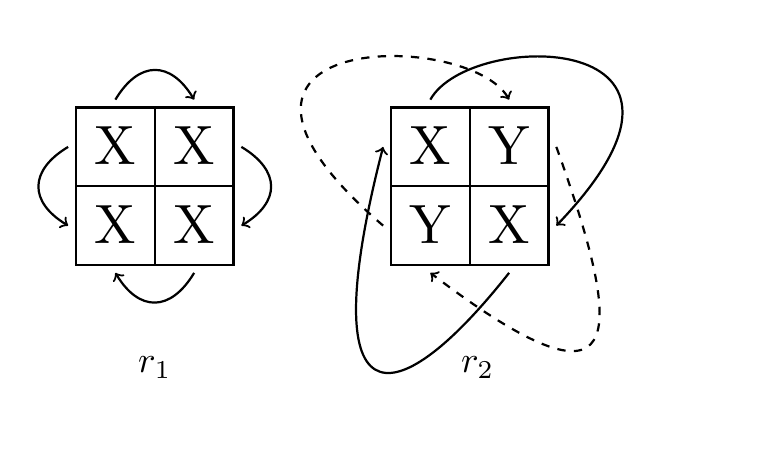
\begin{tikzpicture}

\draw[thick] (-2,4) rectangle (-1,5);
\draw[thick] (-2,5) rectangle (-1,6);
\draw[thick] (-1,5) rectangle (0,6);
\draw[thick] (-1,4) rectangle (0,5);

\draw (-1.5,6) node[anchor=north, scale=2] {X};
\draw (-1.5,5) node[anchor=north, scale=2] {X};
\draw (-0.5,6) node[anchor=north, scale=2] {X};
\draw (-0.5,5) node[anchor=north, scale=2] {X};

\draw[thick,->] (-1.5,6.1) .. controls (-1.2,6.6) and (-0.8,6.6) .. (-0.5,6.1);
\draw[thick,->] (0.1,5.5) .. controls (0.6,5.2) and (0.6,4.8) .. (0.1,4.5);
\draw[thick,->] (-0.5,3.9) .. controls (-0.8,3.4) and (-1.2,3.4) .. (-1.5,3.9);
\draw[thick,->] (-2.1,5.5) .. controls (-2.6,5.2) and (-2.6,4.8) .. (-2.1,4.5);

\draw[thick] (2,4) rectangle (3,5);
\draw[thick] (2,5) rectangle (3,6);
\draw[thick] (3,5) rectangle (4,6);
\draw[thick] (3,4) rectangle (4,5);

\draw (2.5,6) node[anchor=north, scale=2] {X};
\draw (2.5,5) node[anchor=north, scale=2] {Y};
\draw (3.5,6) node[anchor=north, scale=2] {Y};
\draw (3.5,5) node[anchor=north, scale=2] {X};

\draw[thick,->] (2.5,6.1) .. controls (3,7) and (6.5,7) .. (4.1,4.5);
\draw[dashed,thick,->] (4.1,5.5) .. controls (5,3) and (5,2) .. (2.5,3.9);
\draw[thick,->] (3.5,3.9) .. controls (2,2) and (1,2) .. (1.9,5.5);
\draw[dashed,thick,->] (1.9,4.5) .. controls (-1,7) and (3,7) .. (3.5,6.1);

\draw (-1,3) node[anchor=north, scale=1.33] {$r_1$};
\draw (3.1,3) node[anchor=north, scale=1.33] {$r_2$};

\end{tikzpicture}

\end{document}